Recent work in the computer graphics and vision sectors have focused on developing digital tools for reconstructing, tracking, and evaluating human motion using visual input. More specifically, these digital tools that are easier and much cheaper to use, than mocap suits, and in the near future these methods have the potential to surpass the current technology that we talked about in the previous sections. At the moment, the resulting quality of these tools is not as good as the current technology, but many scientists propose state-of-the-art approaches in order to improve them.\\  

 \begin{figure}[h]
	\centering
	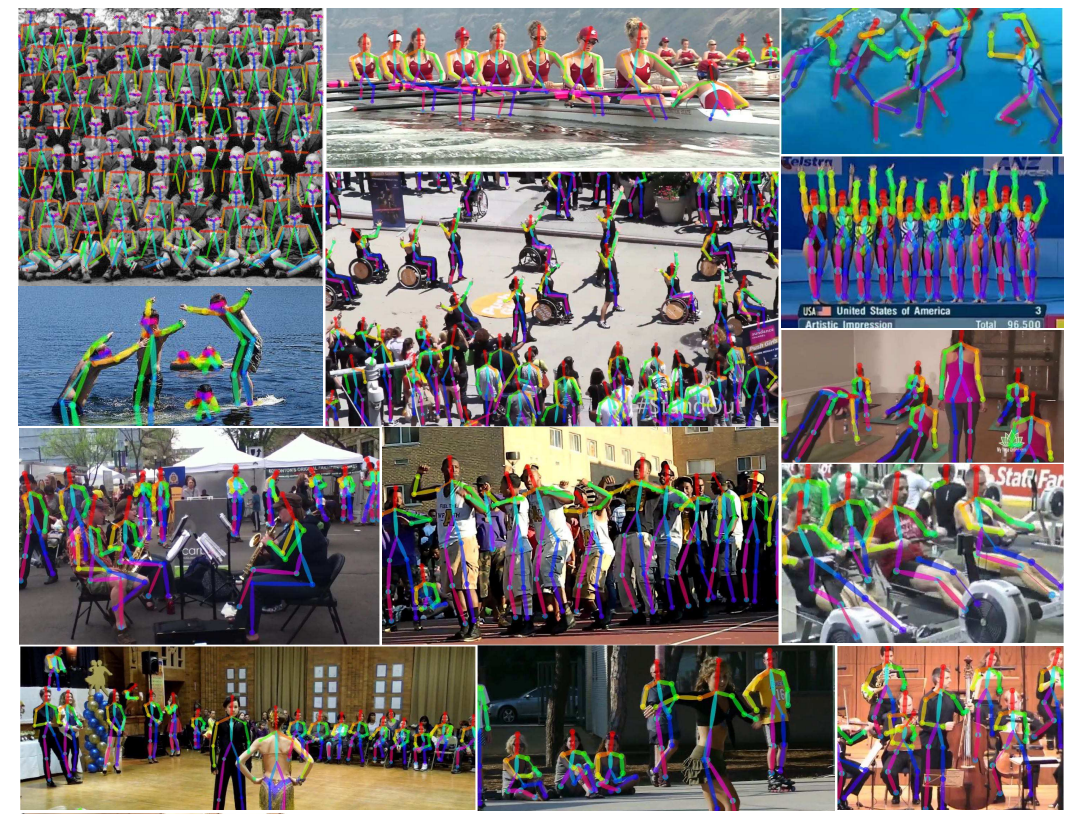
\includegraphics[width=0.6\textwidth]{figures/background/2D.png}
	\caption{\href{https://openaccess.thecvf.com/content_cvpr_2017/papers/Cao_Realtime_Multi-Person_2D_CVPR_2017_paper.pdf}
	{2D Multi-Person high accuracy human Pose estimation}}
\end{figure}

Reconstructing 3D human poses from real-world images in a variety of indoor and outdoor scenarios has a wide range of applications in entertainment, environmental awareness, and human-computer interaction. There are some ways to achieve that, but we will focus more on a specific procedure that estimates 3D human poses from a list of images or a video. Firstly, we will extract the 2D human poses from each image using some well-known Neural Networks specifically trained for this job. In particular, deep neural networks \cite{OpenPose,HrNet,AlphaPose} have revolutionized  2D pose estimation, producing accurate predictions even for poses with self-occlusions. These Neural Network can estimate the 2D human Pose in Real-Time with  high accuracy. These networks were trained with COCO dataset,  which contains over 200, 000 images and 250, 000 person instances labeled with 17 keypoints that are very easily recognisable. Even though the main difference in these network is the architecture and the training the 2D human Pose estimation, is very close. The main difference is the speed of the model and the hardware requirements of each model.\\

\pagebreak

 \begin{figure}[h]
	\centering
	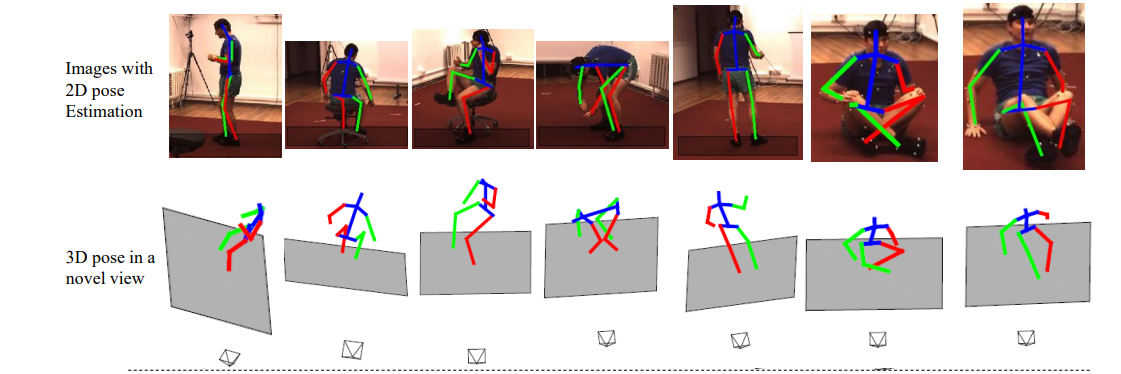
\includegraphics[width=1\textwidth]{figures/background/2D&3D.png}
	\caption{\href{https://arxiv.org/pdf/1612.06524.pdf}
	{2D and 3D human Pose difference in estimation}}
\end{figure}

In the last decade, the research community has paid close attention to inferring the 3D human pose from images or video. All the following studies \cite{Exploiting temporal information for 3D pose estimation,3D Human Pose Estimation from Deep Multi-View 2D Pose,3D Human Pose Estimation Using Convolutional Neural Networks with 2D Pose Information,3D Human Pose Estimation = 2D Pose Estimation + Matching}are proposing a deep neural network that can estimate 3D human poses  from a sequence of 2D human poses. Even though that each paper, proposes a different neural network architecture, all of them uses Human3.6M dataset and some of them, add to the training some other smaller datasets for further improvement of the results.\\

 \begin{figure}[h]
	\centering
	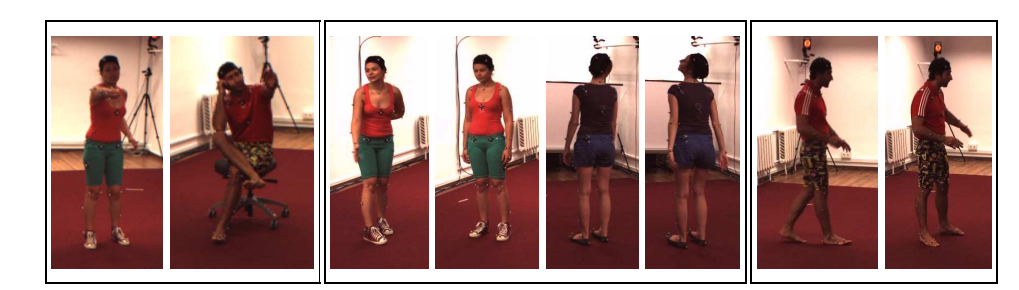
\includegraphics[width=1\textwidth]{figures/background/human36M.png}
	\caption{\href{https://vision.imar.ro/human3.6m/pami-h36m.pdf}
	{Examples of human poses in the Human3.6M dataset}}
\end{figure}

Recently, there has been some interest in systems whose components are trained using datasets of human motion capture . More specifically, a well-known and most used dataset is Human3.6M \cite{Human3.6M} which is a dataset of 3.6 million accurate 3D human poses collected by recording the performance of 5 female and 6 male subjects from four different perspectives in order to train realistic human sensing systems and evaluate the next generation of human pose estimation models and algorithms. \\



